\documentclass{article}
\usepackage{graphicx}
\usepackage{subcaption}
\usepackage{tikz}
\usepackage{hyperref}
\usepackage{fancyhdr}
\usepackage[headheight=30pt, top=1in, bottom=1in]{geometry}
\usepackage[backend=biber, style=ieee]{biblatex}


\title{Research Proposal:\\Surface Analysis of Used Mechanical Heart Valves\\for Microcracks and Defects Detection\\}
\author{Defne Korkmaz\thanks{RWTH Aachen University} \and Priv.-Doz. Dr. Steffen Brinckmann\thanks{Jülich Forschungszentrum}}
\date{\today}

\addbibresource{reflist.bib}

\pagestyle{fancy}
\fancyhf{} % Clear all header/footer content
\fancyhead[C]{\includegraphics[width=0.2\textwidth]{rwthlogo.png}\hfill\includegraphics[width=0.2\textwidth]{jülichlogo.png}}
\renewcommand{\headrulewidth}{1pt}
\fancyfoot[C]{\thepage} % Page number in the center
\renewcommand{\footrulewidth}{1pt}
\begin{document}
\maketitle
\vfill
\pagebreak
\tableofcontents
\pagebreak
\section{Introduction}
Mechanical heart valves are crucial devices that save thousands of lives each day. Despite their seemingly simple structures, the research and engineering that goes into the design and manufacturing of these devices is extensive. Although these devices are crafted to be nearly flawless, after years of use in a patient's vascular system, imperfections, and surface defects can arise. Sometimes, after many decades of use, the valves need to be replaced. Some of the main factors limiting the valve's performance and service life are the roughening of the surface and the generation and propagation of microcracks. 
\\\\A problem called "cavitation erosion" is identified in some research.\cite*{zhang1995} \cite*{wu2001} This is a situation where pressure differences cause the explosion of oxygen bubbles. This not only reduces the surface quality of these valves but also leads to the initiation of microcracks. In another study conducted in 1998 \cite*{barmada1998} (where 17 valves are examined, most of them being demonstration valves; they only have a few valves that have been used, with the longest usage being 4 years), they correlate the deterioration of valve surface quality with the risk of hemolysis. For instance, they look at the roughness of the valve's thin edge, known as the "knife side." They find that valves removed from patients with complaints of hemolysis have a very rough surface in this area.
\\\\In another study from 2001, \cite*{wu2001} a significant relationship between "cavitation damage" and the lifespan of the valves is emphasized again. Local stresses, prolonged cyclic loading over the years, and cavitation damage can all reduce the valve's lifespan in various ways. One of these is triggering hemolysis due to a decrease in surface quality or the formation of thrombi which usually begins from the hinges, as described in a paper from 2012 \cite*{bonou2012}, and more rarely, the valve's fragmentation and detachment as described in a paper from 2019.\cite*{vansteenbergen2019}
\\\\Consequently, the structural integrity of the valve is of utmost importance. Even valves that appear intact to the naked eye have numerous surface defects. These surface defects lead to various issues, including hemolysis, thrombus formation, and even the fragmentation of the valve.

\section{Motivation}
Motivated by patient safety and medical innovation, my proposed research on "Surface Analysis of Used Mechanical Heart Valves for Microcracks and Defects Detection" aims to uncover wear mechanisms that compromise valve performance. Rooted in my father's cardiologist expertise, I'm intrigued by the extent of microcracks on used heart valves and the potential link between service life and valve depreciation. This interdisciplinary study merges materials engineering and medical insights, exemplifying collaboration's potency in solving real-world challenges. With practical implications in heart valve design and testing, this research echoes my commitment to advancing medical science through interdisciplinary excellence.



\section{Background and Literature Review}
\subsection*{Introduction to Mechanical Heart Valves}
Mechanical heart valves have been around for half a century now. Over the years, many heart valves have been designed and implanted into patients. The key positions for these implants are the aortic and mitral positions.\cite*{hutchison2011} The valves can be either fully mechanical or bioprosthetic. Depending on the target position and the patient's condition, either mechanical or bioprosthetic valves may be used. The mechanical valves are often made of stainless steel, titanium, or carbon-coated materials. These are more durable than bioprosthetic valves. The bioprosthetic valves are often made of porcine or bovine tissues integrated with stainless steel, titanium, or carbon-coated materials.\cite*{venkatesh2013} Bioprosthetic valves can be preferred in some patients when the intake of anticoagulant medication is problematic.
\\Mechanical heart valves come in different shapes and sizes. Depending on the price set by the manufacturer, or availability the choice of valves is somewhat more flexible when it comes to in situ application. Most valves used contemporarily perform well for decades after implantation even though they are mostly coupled with anticoagulation therapy throughout the patients' lives. From an engineer or materials scientist's point of view, it is important to consider the material composition and geometry of the valves more in-depth, which will be done in the next sections.\\
\subsection*{Material Composition and Structure}
The main parameters that are important in mechanical heart valves are biocompatibility, wear resistance, radioopacity, and durability. Most valves use tungsten-impregnated pyrolytic carbon over graphite, titanium coated with pyrolytic carbon, and barium-containing silastic polymer.\cite*{hutchison2011} There are more than seventy different cardiac valves available in the market, but they can be categorized under four main types. These are Caged Ball Valves, Tilting Disk Valves, Bileaflet Valves, and Bioprosthetic Valves.\cite*{venkatesh2013} Björk-Shiley valve acquired for this research proposal, is one of the most studied valves and it is a tilting disk valve. The Medtronic valve acquired for this research is a type of leaflet valve. Both valves are made of pyrolytic carbon-coated titanium alloys.

\begin{figure}
    \centering
    \includegraphics[width=0.8\textwidth]{björkshileyvalve.png}
    \caption{Björk-Shiley Valve. \cite*{björk1969}}
    \label{fig:björkshileyvalve}
\end{figure}
\vspace{1pt}

\subsection*{Complications}
There are some complications that arise from prosthetic heart valves. These are the growth of pannus tissue, infective endocarditis, thrombosis, and hemolysis.\cite*{roudaut2007} \cite*{barmada1998} The pannus tissue is a connective tissue that grows onto the heart valves eventually hindering its movement. Infective endocarditis is a medical issue that usually occurs as a result of the bacterial infection of the heart valve and the surrounding tissue triggered by the cardiologic/surgical operation. The last two issues, however, are more related to the surface quality and structural integrity of the mechanical heart valves. The roughened surface of the valve provides a more suitable environment for thrombosis to occur, increasing the risk of blood clot formation. Furthermore, the presence of microcracks in the valve structure can contribute to the formation of thrombosis and also compromise the durability of the prosthetic. In some extreme cases, the formation and propagation of microcracks can reach such a level that the leaflet/leaflets of the heart valve break off and cause complete valve failure, causing significant problems by embolization in the arterial tree.\cite*{vansteenbergen2019}
\subsection*{Methods of Detecting and Monitoring Microcracks}
There are several methods to detect the presence of faults in the heart valves. Some of these methods are echocardiography, cardiac tomography, x-ray examination, fluoroscopy, or suspicion raised from certain patient symptoms similar to heart valve disease like shortness of breath, feeling dizzy and tired, etc. Medical professionals can also use a stethoscope to listen to the sound of the heart valves and detect a decrease in the valve sound, which would mean reduced functionality. The most extensive way, however, is only possible after the removal of the mechanical heart valves and inspection under a light microscope (LM), where the presence and extent of microcracks can be visually examined, later scanning electron microscopy (SEM) and possibly even fringe pattern interferometry (FPI).\cite*{barmada1998} FPI will give insight into the roughness of the surface.

\subsection*{Common causes of Microcracks}
Microcracks and other surface defects on the valves arise after years of operation. Certain parameters in the body like pressure inside the veins, repeated load, and friction can contribute to the formation and progression of microcracks in mechanical heart valves. One of the important phenomena that add to surface defects and microcracks is the cavitation potential of the blood.\cite*{zhang1995} This is observed when the local pressure of the blood drops below the vapor pressure, causing the rapid formation of bubbles that implodes upon reaching areas of higher pressure. This causes shock waves on nearby surfaces, in this case, the surface of the mechanical heart valve.\cite*{wu2001} These shock waves contribute to the formation of microcracks and erosion of the surface of the valves.


\section{Research Objectives}
\begin{enumerate}
    \item Conduct literature search
    \item Acquire sterilized samples
    \item Prepare the samples, remove suture rings or any extra components
    \item Initial analysis under an optical microscope
    \item Cut and polish the samples
    \item Analyze under an optical microscope
    \item Document findings, collect images
    \item Discuss if there is a correlation between the service life and the amount and extent of surface defects on the valves
    \item Report findings
\end{enumerate}
\pagebreak
\section{Sample Collection and Preparation}
Two samples have already been acquired, and the brand and service life of these samples are summarized in the table below.

\begin{center}
    \begin{tabular}{|c|c|c|c|}
        \hline
        Sample & Brand & Material & Service Life \\
        \hline
        1 & Medtronic\cite*{medtronic_image} & Carbon coated titanium & 4 days \\
        \hline
        2 & Björk-Shiley\cite*{björk1969} & Carbon coated titanium & 35 years \\
        \hline
    \end{tabular}
\end{center}

Approximately 10 more samples will be acquired. These samples are expected to have service lives distributed evenly in the range from 1 year to 40 years.
The servie duration of the valves will be noted and each valve will be photographed and labelled.
If necessary, other information regarding the removed heart valves may be collected.


\section{Timeline and Work Plan}
Below is a timeline showing all the past and future milestones of this proposed study.\\
\vline
\\Progress to be made in 2023:
\begin{figure}[h]
    \centering
    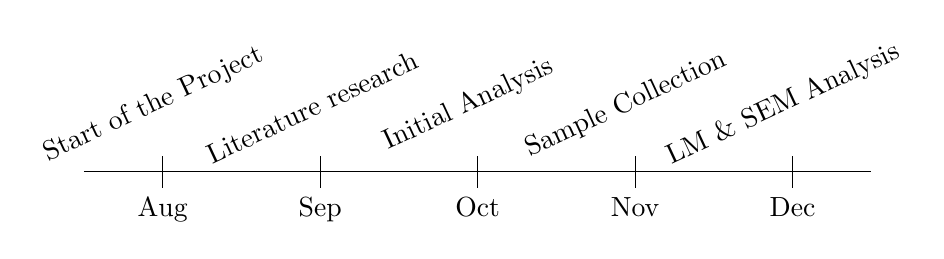
\begin{tikzpicture}
        \draw (0,0) -- (10,0);
        \foreach \x/\month/\labeltext in {1/Aug/Start of the Project, 3/Sep/Literature research, 5/Oct/Initial Analysis, 7/Nov/Sample Collection, 9/Dec/LM \& SEM Analysis}{
            \draw (\x,0.2) -- (\x,-0.2) node[below] {\month};
            \node[above, rotate=25] at (\x,0.6) {\labeltext};
        }
    \end{tikzpicture}
    \caption{Project Timeline - 2023}
\end{figure}
\\Progress to be made in 2024:
\begin{figure}[h]
    \centering
    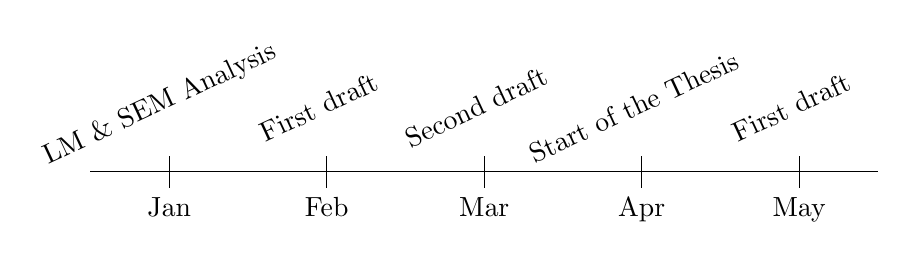
\begin{tikzpicture}
        \draw (0,0) -- (10,0);
        \foreach \x/\month/\labeltext in {1/Jan/LM \& SEM Analysis, 3/Feb/First draft, 5/Mar/Second draft, 7/Apr/Start of the Thesis, 9/May/First draft}{
            \draw (\x,0.2) -- (\x,-0.2) node[below] {\month};
            \node[above, rotate=25] at (\x,0.6) {\labeltext};
        }
    \end{tikzpicture}
    \caption{Project Timeline - 2024}
\end{figure}
\section{Ethical Considerations}
The proposed research does not entail any significant ethical considerations. The focus of the study is solely on the material analysis of used replacement heart valves and these valves are obtained anonymously, without any personal or sensitive data linked to the former owners of these implants. Only medical information related to these implants are the following: the brand and model of the implant, and the time spent in the patient's body. Nonetheless, adherence to scientific integrity will always be a priority throughout the research.

\section{Conclusion}
This research proposal outlines the plan to study the correlation between the service duration and the surface quality of used mechanical heart valves. Following a timeline, it is aimed to achieve the goals through research, sample collection, and analysis in a systematic manner. It is aimed to provide insights into heart valve performance, contributing to a better understanding of the incidence of surface defects on mechanical heart valves. This will help with understanding the most defect-prone regions of the heart valves and ultimately develop more advanced methods or tools to quantify/characterize the surface defect on removed heart valves.


\pagebreak
\printbibliography
\end{document}